\documentclass[../main/main.tex]{subfiles}

\newdate{date}{29}{10}{2020}


\begin{document}

\marginpar{ \textbf{Lecture 9.} \\  \displaydate{date}. \\ Compiled:  \today.}

We recall now one of the most important result of the last lecture: if the network is large enough, for \( N \rightarrow \infty  \), the \textbf{epidemic threshold} tends to zero:
\begin{equation}
    \beta_c \xrightarrow{N \to \infty} 0
\end{equation}
Moreover, the epidemic threshold for IBMF depends on the largest eigenvalue of the adjacency matrix $\Lambda_{max}$.
The last relations which contain \( \beta _c \) for IBMF and DCBMF, can tell us more about the accuracy of the model: \textbf{DBMF} is accurate only in the proximity of the epidemic threshold, while \textbf{IBMF} is accurate for the entire epidemic diagram. See the figure \ref{fig:09_1}. 

\begin{figure}[h!]
\centering
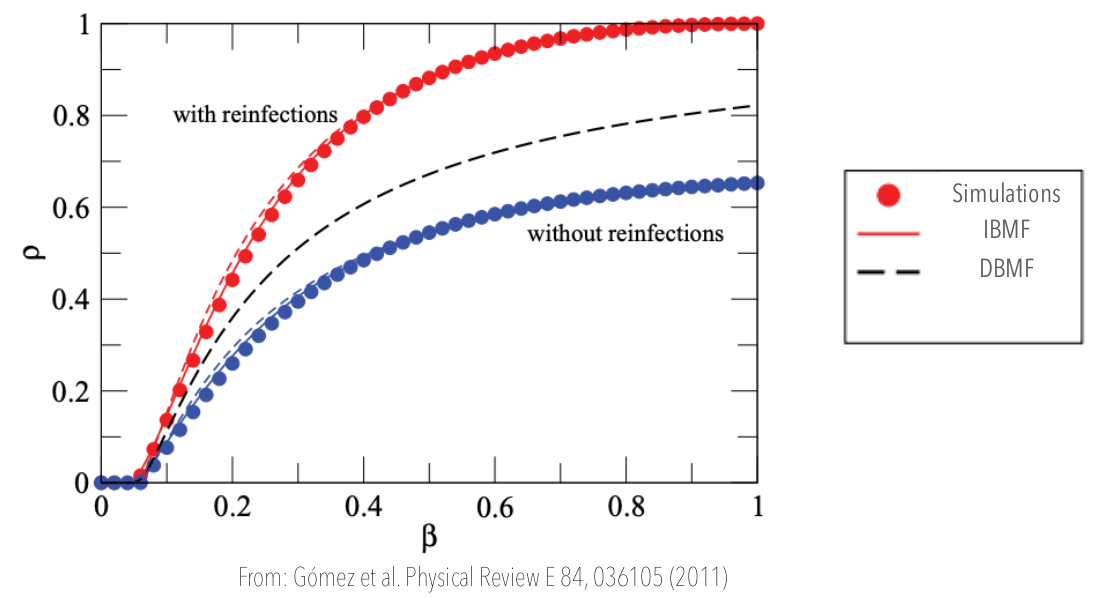
\includegraphics[width=0.7\textwidth]{../lessons/image/09/image01.png}
\caption{\label{fig:09_1} The quenched mean field (IBMF) curve follows exactly the simulation, while DBMF the is precise only around the epidemic threshold.}
\end{figure}

We want now to discuss what are the reasons behind this important result. Since we know there is a strong connection between these two theories, it would be of our interest to derive DBMF from IBMF. Once again, we shall repeat that in \textbf{annealed networks} we are not considering a single network but an \textbf{average} of all the \textit{possible random networks} that can be generated \textit{from a degree distribution}. Instead, in the \textbf{quenched networks} we pick a particular \textbf{one}, and we compute the result for \textit{that specific network}. Then, nothing prevents us to run our model on that network and iterate multiple times.

Let us try to characterize the \textbf{annealed network}, in particular we want to see the \textit{adjacency matrix} looks like. In this case, the \textbf{adjacency matrix} is a \textbf{weighted matrix}, whose general form is:
\begin{equation*}
  \bar{A}_{ij} = \frac{k_j P(k_i|k_j)}{N P (k_i)}
\end{equation*}
and for \textbf{random networks} becomes:
\begin{equation*}
  \bar{A}_{ij} = \frac{k_i k_j}{N \expval{k} } = \frac{k_i k_j}{2 L}
\end{equation*}
where the probability  \(  P(k_i|k_j) \) of picking a random node is \( k_j \). This is the number of trials we have available in order to create this specific connection, over all the possible connections that the network can return.

Then, we have now simply to substitute the last result in the expression \ref{eqn:q_prod} of \( q_i \):
\begin{equation*}
  q_i = 1 - \prod_{j=1}^{N} \qty[1 - \beta \frac{k' P(k'|k)}{N_{k'}} \rho _j]
\end{equation*}
And starting from individual nodes and heading towards more general degree classes:
\begin{equation*}
  \dot{\rho }_k = - \mu \rho _k + (1- \rho _k)\left[ 1 - \prod_{k'} \qty[1 - \beta \frac{k P(k'|k)}{N_{k'}} \rho _k]^{N_{k'}} \right]
\end{equation*}
this is the most general expression that we can obtain for DBMF.
The multiplication can be replaced by a sum, only if assuming that \( \beta \rho _k \ll 1 \):
\begin{equation*}
  \dot{\rho }_ k = - \mu \rho_k + \beta k (1-\rho_k) \sum_{k'}P(k'|k)\rho_k'
\end{equation*}
And recalling that the expression for $\Theta_k = \sum_{k'}P(k'|k)\rho_{k'}$:
\begin{equation*}
   \dot{\rho }_ k = - \mu \rho:k + \beta k (1-\rho_k) \Theta_k
\end{equation*}
That actually is accurate only under the assumption \( \beta \rho _k \ll 1 \). But one should note that this is exactly what is depicted in the plot above! Hence, we are able to switch from IBMF to DBMF and, in this way, we can even explain why there is such difference in the accuracy between the two models.

\subsection{IBMF and pair approximation}
Let us make a very brief overview about what means to \textbf{cut down} the chain to \textbf{pair approximation}.
Up to now, all the models we have seen were cut at the \textit{individual level}. Now, instead, let us consider the joint probability of being infected, given that we we susceptible and given that a neighbor of ours was infected. We look for an approximation for this joint probability, and this time we choose to cut the chain at the level of a single link $(i,j)$. We want to see actually how $P\{\sigma_i(t) = 0\ ,\   \sigma_j (t) = 1\}$ changes in the equation for $\dot{\rho}$.
Hence we obtain:
\begin{equation*}
  \dv{}{t} \rho (i,t) = - \mu \rho (i,t) + \beta \sum_{j}^{} A_{ij} \rho (j,t) - \beta \sum_{j}^{} A_{ij} \mathbb{E} \qty[X_i (t) X_j (t)]
\end{equation*}
where \(  \mathbb{E} \qty[X_i (t) X_j (t)] \) is the two nodes expectation probability to be infected. 

However, we need to look for an expression for the $\binom{N}{2}$ equations for \(  \mathbb{E}  \qty[X_i (t) X_j (t)] \), since we have to take into account one expression for each node multiplied all possible link we can have in the network.
The main idea is:
 \begin{equation*}
  \dv{}{t} \mathbb{E} \qty[X_i (t) X_j (t)] =
  \end{equation*}
  
  \begin{equation*}
  = - 2\mu \mathbb{E} \qty[X_i (t) X_j (t)] + \beta \sum_{k}^{} A_{jk} \mathbb{E} \qty[X_j (t) X_k (t)] - \beta \sum_{k}^{} (A_{ij} + A_{jk}) \mathbb{E} \qty[X_i (t) X_j (t) X_k (t)]
\end{equation*}
Let us analyze the terms on the rhs. The first one is the \textbf{recovery term} and needs both of \textit{them to be infected}. On the other hand the second and third terms are the \textbf{infection terms}, where either one of the node is already infected and the susceptible term gets infected from any other neighbour. The last term has to be put in order to discard the three nodes expectations, and here comes the need for an \textbf{approximation}, namely a \textbf{closure}.

The most used closures used in the literature are:
\begin{equation*}
    \mathbb{E} \qty[X_i (t) X_j (t) X_k (t)] =  \mathbb{E}[X_i(t) X_j(t)]  \mathbb{E}[X_k(t)] 
\end{equation*}
where in this case the third term we factorize out is the \textit{mean-field} term.Alternatively:
\begin{equation*}
    \mathbb{E} \qty[X_i (t) X_j (t) X_k (t)] = \frac{\mathbb{E}[X_i(t) X_j(t)] \mathbb{E}[X_j(t) X_k(t)] }{\mathbb{E}[X_i(t) X_k(t)] }
\end{equation*}
where the second is similar to the first but we are considering the two extremes and the probability that \( j \), the node in between, is infected.



\chapter{Epidemic spreading on networks: more advanced models}

\section{Non-Markovian Epidemic Spreading}

Despite it is difficult to find it discussed in literature, we surely need to take into account that \textbf{both} the \textbf{infection process} and \textbf{recovery process} in reality \textbf{DO NOT} have a constant rate. 

Up to now, we have assumed the other way around: at each time step the probability of being recovered is always the same, no matter how much we have stayed in the \textit{Infected} compartment. Therefore, our process is \textbf{memoryless}. Since the jumps are memoryless, we can characterize our problem as if we were running a Markov chain. Let us recall what is its \textbf{main property}: the \textbf{jump probability does not depend on time}. Hence, it is not needed to take into account the time we spent there, and so time spent inside each compartment follows an \textbf{exponential distribution}.
We refer to the average time that we spend there as \( \tau = \frac{1}{\mu }\) and the underlying pdf is shown in \ref{fig:09_2}:
\begin{equation*}
  P(x) = \tau e^{- \tau x}
\end{equation*}

\begin{figure}[h!]
\centering
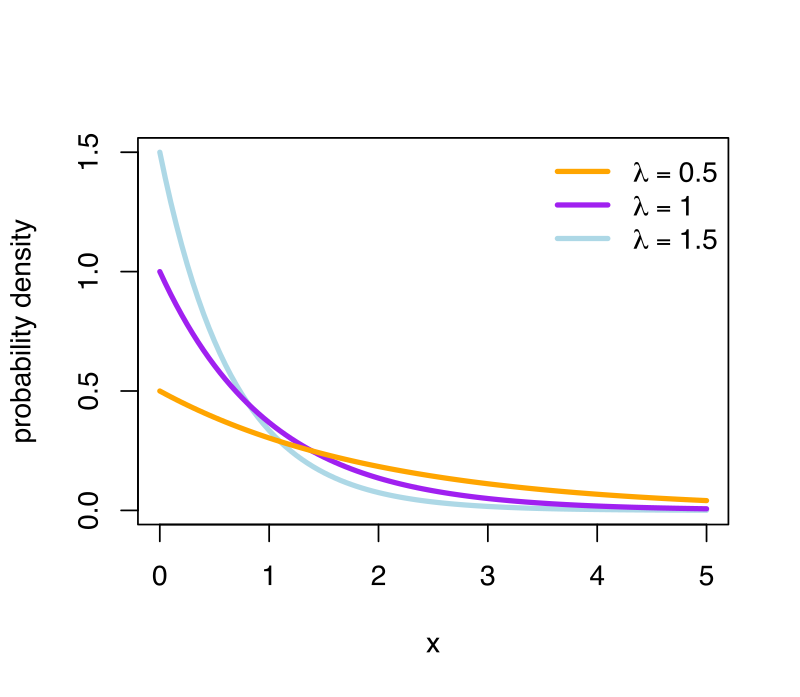
\includegraphics[width=0.7\textwidth]{../lessons/image/09/image02.png}
\caption{\label{fig:09_2} Exponential probability density function for different $\lambda = \tau$. Note as the most probable value is when we start our observation, namely at the moment in which $x=0$. }
\end{figure}


We want now to discuss what are the implications these assumptions we have made so far. The most immediate one is that the \textbf{mode}, namely the most probable duration of being infected, is \textit{null}. Obviously, the "height" does depend on the mean value, but in any case the most probable moment when we can make the jump is at the beginning of our observation window (see fig \ref{fig:09_2}). Obviously, this is something that is \textbf{not realistic}. If we got influenza, we do expect to spend at least some time infected, and we do not expect the probability to decrease wrt time. If we wanted to see how infectious periods are distributed in real life, it is indeed something quite different, and do not behave like an exponential. For any disease, we can know (almost) exactly when it starts, but we are obviously not aware when it is going to end. For instance, let us consider the plot for 2009 H1N1 Influenza. For this specific strain of influenza, the \textbf{mode} is around 2 days and an half, so it is not 0 as we would expect from an exponential!

\begin{figure}[h!]
\centering
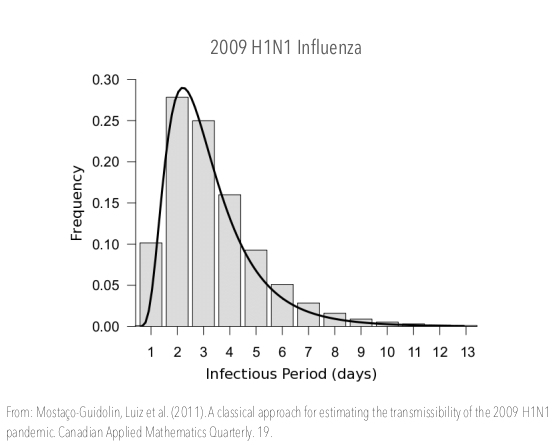
\includegraphics[width=0.7\textwidth]{../lessons/image/09/image03.png}
\caption{\label{fig:09_3} Infectious period distribution for the 2009 H1N1 influenza. One should note how it does not follow and exponential, therefore the mode is not located at $x=0$, hence the approximation of the recovery rate constant in time is not realistic.}
\end{figure}


However, we can make estimates also for Covid-19, see figure \ref{fig:09_4}.

\begin{figure}[h!]
    \centering
    \subfloat[Some of the inferred recovery distributions for the Covid-19 disease.]
        {
            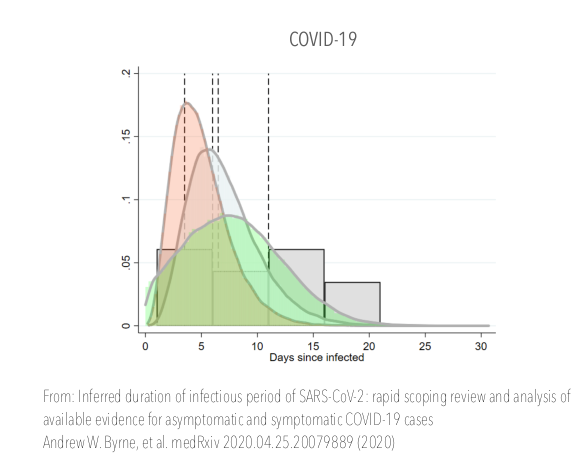
\includegraphics[width=.45\textwidth]{../lessons/image/09/image04a.png}
            \label{fig:09_4a}
        }
    \qquad
    \subfloat[Probability distributions for the recovery rate, note as this is not unique and it may vary according to data scientists are looking at. However, this is not an exponential at all]
        {
            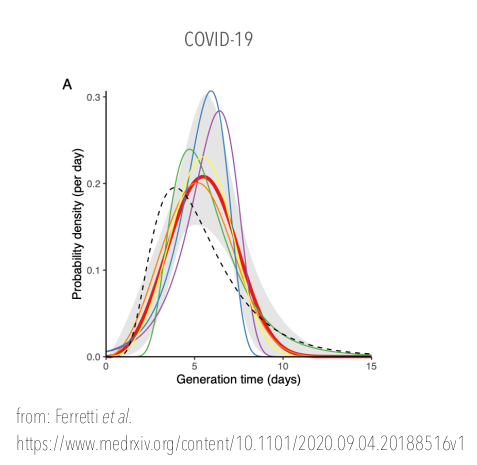
\includegraphics[width=.45\textwidth]{../lessons/image/09/image04b.png}
            \label{fig:09_4b}
        }
    \caption{\label{fig:09_4}}
\end{figure}

An observable easier to measure is the so called \textbf{serial interval}, namely the one that is between the onset of symptoms from an individual, to the onset of symptoms for another individual. Despite this is just an \textbf{approximation}, it still can tell us some useful information.

At this point we should have been convinced by last considerations that these kind of diseases are \textit{not Markovian}. Hence, the \textbf{recovery times depends on the time} we spend in that specific compartment. Now another problem arises, that is how to model this "non Markovianity".
The family distribution that better describes our empirical data is the \textbf{Gamma distribution}:
\begin{equation*}
  P(x) = \frac{1}{\Gamma (k) \theta ^k} x^{k-1} e^{- \frac{x}{\theta }}
\end{equation*}
the curve in fig. \ref{fig:09_5} starts to resemble somehow our observations. A similar family of distributions is the so called \textbf{Erlang distributions}, where the factorial replaces the Gamma function in the denominator.

\begin{figure}[h!]
\centering
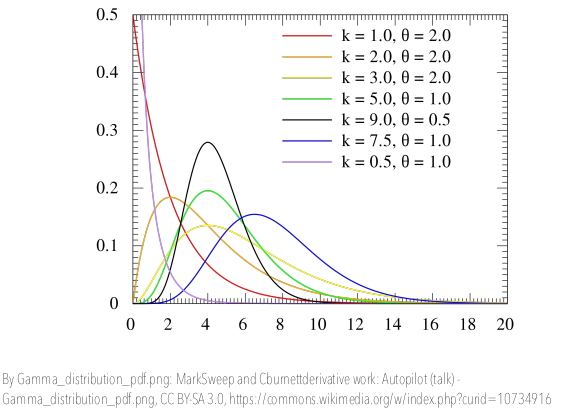
\includegraphics[width=0.5\textwidth]{../lessons/image/09/image05.png}
\caption{\label{fig:09_5} Gamma distribution for different changes of parameter. }
\end{figure}

Note that both distribution families introduced so far are able to reproduce quite well the shape of histogram, found by mean of empirical data.

We need now to discuss on how to include this \textbf{non-markovian} behavior into the \textbf{classical} epidemiological \textbf{models} we have introduced so far. One should note that, when analyzing them, we were assuming the markovian property.
A \textbf{first} approach is the following. Let us consider a \textit{trick} for the \textbf{infectious period}. We want to exploit the theoretical result that the sum of exponential random variables obeys to a gamma distribution. Specifically for our model, instead of considering only one transition with a constant rate (i.e. a single exponential distribution), we are going include \textbf{many transitions}, every one with its own rate. Therefore instead of having only a single infectious state, there will be many. Individuals will be able to move sequentially from one compartment to another. In this way, they will be forced to spend \textbf{at least some time infectious} before being recovered. Hence, we obtain a markovian model. Despite we are forced to spend some time infected before being recovered, the underlying model is still markovian. The only constraint is that we are imposing that these \textbf{stages} must be \textbf{sequential}.


Writing formally the equations with these last considerations:
\begin{equation*}
    \dv{s}{t} = -\beta s i \qquad \dv{i_1}{t} = \beta s i - K \mu i_1 \qquad \dv{i_2}{t} = K \mu i_1 - K \mu i_2 \quad ... \quad \dv{r}{t} = K \mu i_K
\end{equation*}
Where we introduced $K$ different infected compartments $ i = \sum_{k=1}^K i_k$. Hence a generic transition rate for each I transition is \( K \mu  \). 

The infectious period distribution is the sum of these "intermediate" exponentially distributed random variables, namely:
\begin{equation*}
    P(\tau) = \frac{(\mu K)^K}{\Gamma (K)} \tau^{K-1} e^{-\mu K \tau}
\end{equation*}
which is a gamma distribution.
Some limiting cases are:
\begin{itemize}
\item if \( K=1 \), we obtain an \textit{exponential} distribution;
\item if \( K \rightarrow \infty  \) fixed, we obtain a \textit{delta} distribution.
\end{itemize}
And this conclude the first approach in order to deal with non-markovian problems.

A \textit{second} approach, which is \textbf{more general}, allows us to include \textit{non-markovian} property both in \textbf{recovery} and \textbf{infections}.
We want to discuss whether there is the possibility to write a more general model on networks as possible. Practically, this is feasible, despite at some points some sort of approximations will be needed. In order to do this, we have to slightly change our point of view and modify our approach: instead of probabilities, now we will be considering \textbf{events}. The idea is that we need to \textbf{model infections} and \textbf{recoveries} according to \textbf{two random numbers}, which are drawn from a distribution as general as possible.
Every time we extract a random number, which actually represents the time when we recover (i.e. the time we will spend as infected). This is defined as \( R_i (t) \). Then, an other random number need to extract is \( M_{ij} (t) \) which represents the number of trials that \( i \) makes while trying to infect node \( j \). This is to be repeated for all the neighbours.
The sequence generated will be the following:
\begin{equation*}
  T_{ij}^{(1)} \leqslant T_{ij}^{(2)} ... \leqslant T_{ij}^{(M_{ij}(t))} \leqslant R_i(t)
\end{equation*}
where \(  T_{ij}^{(1)} \) is the first time at which node $i$ tries to infect node $j$, then we have the second time, \(  T_{ij}^{(2)} \) and so forth. Hence, the \textbf{transmissibility} of a disease depends on how many trials we have available to infect.

The \textbf{algorithm} for infections looks like the following: once we have fixed a node $i$, we \textit{draw} a number $R_i(t)$ that is \textit{not} going to change unless we consider the following time step $t+1$. One should note that $R_i(t)$ is the time at which node $i$ will recover. Later, we consider one of its neighbours, for instance $j$ and draw the number that defines how many attempts $i$ will have in order to infect $j$: $M_{ij}(t)$. For each of these attempts, we will draw $T_{ij}^{(n)}$ and if the latter is less that $R_i(t)$ the node $j$ will be considered to have been infected. Otherwise, we keep going extracting  $T_{ij}^{(n)}$, with the constraint that $n$ must be at most $M_{ij}(t)$. We iterate this procedure for each of the neighbors of $i$ and see which nodes are going to be infected next time step $t+1$.
At $t+1$, then, we fix another node $k$ that is infected and draw $R_k(t+1)$, choose a node $j'$ among its neighbors, draw $M_{kj'}(t+1)$ and repeat what we have stated before.
One last remark is that \( R \) and \( M \) can follow \textbf{any distribution} and not only the exponential one. How we extract $T$ is not important, because the only point that matters is how $R$'s and $M$'s are distributed.

Let us make some \textbf{assumptions} in order model these distributions reasonably, and finally try to solve our problem analytically. We can consider both $R$'s (recovery times distribution) and $I$'s (infection times distribution) to be \textbf{peculiar} of the disease, therefore must \textbf{not depend} both on the \textbf{node} and on \textbf{time}. Obviously they should take into account the background information, for instance lockdown, particular restrictions...but momentaneously we will skip this part.

In other words we are just \textbf{reducing} the \textbf{complexity} of our problem by stating that \( R_i(t)  \to  R \) and \( M_{ij}(t) \to  M \). We define the long run probability \( v_i \) to be the \textbf{probability} that node \( i \) is \textit{infected} in the \textbf{steady state}.


Now it is time to build our model. Let us suppose that we are in the \textbf{steady state}, that is to say that there is no more transiency. In the long run, for a period of time $[0,S)$ and $S$ large enough, the number of times that node \( j \) was infected is proportional to \( S \). Therefore we are introducing in our model the property that the number of times that we contract the infection is linear wrt time.
\textit{On average}, the length of each infected period is $\mathbb{E}[R]$ (expected time to recover). Then, in the long run, the \textit{number of times} that node $j$ \textit{has been infected} in a period of length $S$ can be rewritten as:
\begin{equation*}
  \frac{v_j S}{\mathbb{E}[R]}
\end{equation*}

Recall now that for every time step in which node $i$ is infected, it will attempt to infect its neighbour $i$ on average \(\mathbb{E} [M] \) times. \textit{On average}, the \textit{total number} of infection \textbf{attempts} from node $j$ to $i$ in the long run is the following:
\begin{equation*}
    \frac{v_j S\mathbb{E}[M]}{ \mathbb{E}[R] }
\end{equation*}

Now we want to make a \textit{mean-field} assumption. We recall that it refers to the joint probability that $j$ is infected while $i$ is susceptible and allows us to factorize in the following way:
\begin{equation*}
    P[\sigma_i(t) = 0\ ,\ \sigma_j(t) = 1 ] \sim P[\sigma_i(t) = 0] P[\sigma_j(t) = 1 ] = (1-v_i) v_j  
\end{equation*}
Where we replaced the two factors by the probabilities of the respective node for large time intervals.

Let us consider now the number of times which \( i \) actually received the infection from \( j \). \textit{On average}, in the long run, the \textbf{number of successful attempts} made by $j$ to infect its neighbor i $i$ is the following:
\begin{equation*}
S \frac{\mathbb{E}[M]}{\mathbb{E}[R]} v_{j} (1-v_i)
\end{equation*}
That is nothing more than the total number of attempts we computed before, times the probability that node $i$ was not infected.
If we sum over all the neighbors of $i$, we obtain the the \textbf{total number of successful infections} $i$ will receive during time interval $[0,S)$:
\begin{equation*}
  S \sum_{j=1}^{N}  a_{ij} \frac{\mathbb{E}[M]}{\mathbb{E}[R]} v_{j} (1-v_i) = v_i \frac{S}{\mathbb{E}[R]}
\end{equation*}
Where the last equivalence asymptotically holds only in the \textbf{steady state}, and the rhs is the number of infected periods experienced by $i$.
Simplifying last formula we have that:
\begin{equation*}
  v_i = \mathbb{E}[M] (1- v_i) \sum_{j=1}^{N} a_{ij} v_j
\end{equation*}
hence the probability of $i$ being infected depends on the sum over all its neighbours, times the term \( \mathbb{E}[M] \) which is the average number of infection attempts it will experience during that time interval.

This last expression should sound familiar: it is exactly what we obtained from the \textbf{linearization} of the quenched mean field approach (IBMF). The only difference is that before we had:
\begin{equation*}
  \mu \varepsilon_i^* = \beta (1 - \varepsilon_i^*) \sum_{j=1}^N A_{ij}\varepsilon_j^*
\end{equation*}
While now a generic infection term \( \mathbb{E}[M] \) replaces the $\beta$ term in the $IBMF$. This generic infection term therefore encodes all the distributions with the same expected value $\mathbb{E}[M]$. Note that this last result holds \textit{only} in the \textit{steady state} and \textit{do not} depend on the shape of the distribution $M$, but only on its expected value!

Let us briefly discuss the \textbf{implications} for this. One should note that the definition of the distribution $M$ already includes the recovery term $R$, since at the end of the day it sets a "bound" for it:
\begin{equation*}
  T_{ij}^{(1)} \leqslant T_{ij}^{(2)} ... \leqslant T_{ij}^{(M_{ij}(t))} \leqslant \mathcolorbox{yellow}{R_i(t)}
\end{equation*}
Moreover, the expected number of infection events in a Poisson process with intensity $\beta$ and an exponential recovery time whose expectation is $1/\mu$, we can prove that:
\begin{equation*}
    \mathbb{E}[M] = \frac{\beta}{\mu}
\end{equation*}
Last information we can obtain is that the epidemic threshold $m_c$ can be derived from:
\begin{equation*}
    m_c = \mathbb{E}[M_c] = \frac{1}{\Lambda_{max}}
\end{equation*}











\end{document}
